% # COPYRIGHT:
%
% Copyright (C) 2011 Jeremiah Mahler <jmmahler@gmail.com>.
% Permission is granted to copy, distribute and/or modify this document
% under the terms of the GNU Free Documentation License, Version 1.3
% or any later version published by the Free Software Foundation;
% with no Invariant Sections, no Front-Cover Texts, and no Back-Cover Texts.
% A copy of the license is included in the file "fdl-1.3.txt".
%
\documentclass[12pt]{article}
%\usepackage{mslapa}
\usepackage{hyperref}
\usepackage{amsmath}
\usepackage{graphicx}
\usepackage{ulem}
\usepackage{vmargin}
\usepackage{tabularx}
\usepackage{sectsty}
\usepackage{pbox}
\usepackage{bigstrut}
\usepackage{enumerate}
\usepackage{parskip} % add spaces between paragraphs
\input kvmacros % Karnaugh Maps and Veitch charts
%\usepackage{cleveref}
\usepackage{verbatim}

\setpapersize{USletter}
\setmarginsrb{1.0in}{1.0in}{1.0in}{1.0in}{0in}{0.25in}{0in}{0.20in}

\sectionfont{\normalsize}
\subsectionfont{\normalsize}

% configure \bigstrut size
% This configures spacing above and below rows in a tabularx.
%\renewcommand{\bigstrutjot}{6pt}

\renewcommand{\bigstrutjot}{2.0\jot}

\setlength{\parindent}{0in}

\raggedright

\begin{document}

% {{{ Cover Page
\centerline{\bf EECE 144}
\centerline{\bf Fall 2011}
\centerline{\bf}
\centerline{\bf Lab Report \#10}
\centerline{\bf Section 4}
\centerline{\bf 11/9/2011}
% signature area
\begin{center}
\begin{tabularx}{\textwidth}[b]{X l l}
Submitted by: Jeremiah Mahler & & \\
Signature & Printed Name & Date \\
\hline
\multicolumn{1}{|X|}{} & \multicolumn{1}{|l|}{\bigstrut \bf Jeremiah Mahler} & \multicolumn{1}{|l|}{\bf Nov 9, 2011} \\
\hline
\multicolumn{1}{|X|}{} & \multicolumn{1}{|l|}{\bigstrut \bf Marvanee Johnson} & \multicolumn{1}{|l|}{\bf Nov 9, 2011} \\
\hline
\end{tabularx}
\end{center}
% }}}

% {{{ Description/Objectives
\section{Description/Objectives}

The objective of this lab is to design a three bit binary counter
using at least one D flip-flop and at least one JK flip-flop.
And then implement this design in hardware.

\begin{table}[hbp]
\begin{center}
\begin{tabular}[t]{r|cccc|ccc}
n & $Z_2$ & $Z_1$ & $Z_0$ \\
\hline
0 & 0 & 0 & 0 \\
1 & 0 & 0 & 1 \\
2 & 0 & 1 & 0 \\
3 & 0 & 1 & 1 \\
4 & 1 & 0 & 0 \\
5 & 1 & 0 & 1 \\
6 & 1 & 1 & 0 \\
7 & 1 & 1 & 1 \\
\end{tabular}
\end{center}
\caption{The sequence of states for a 3-bit binary counter
where $Z_0$ is the least significant bit.
The counter should following this order and when the end is reached
it should loop to the beginning.}
\label{tbl:tt}
\end{table}

% }}}

% {{{ Procedure
\section{Procedure}
\label{sec:procedure}

The first step is to design the 3-bit counter.
The strategy used here is to first solve the least significant
bit and then proceed to the more significant bits.
This is because the least significant bit does not depend on the
state of any of the higher bits.
The second bit depends on the state of the first bit.
And the third bit depends on the state of the second and
possibly the first.

Here we used one D flip-flop for the first bit and two JK flip-flops
for subsequent bits.
But other combinations are possible.
In fact it is possible to use any register type for any bit position.
It is even possible to implement a JK flip-flop out of a D flip-flop
using only a few additional logic gates.

And after the design is created it will be implemented in hardware.

% {{{ bit Z_0
\subsection{bit $Z_0$, toggle using D flip-flop}
The least significant bit behaves like a "toggle".
When it is triggered by the clock it changes the output ($Q^+$)
to the opposite of its previous state ($Q$).
\footnote{The notation used here denotes $Q$ as the current state and $Q^+$ 
as the next state.}

For the least significant bit, $Z_0$, the relevant states
are given in Table \ref{tbl:dtoggle}.
It can be seen that when $Q$ is $0$ we want the state, $Q^+$,
to be $1$.  And the only way a D flip-flop can produce a $1$ as
an output is if it has a $1$ on its input ($D$).
Similar reasoning can be used for the second row.
To construct a function we need to decide what mapping from $Q$
would produce the values in $D$. 
In this case it is simply $D = Q'$.
What this function means in terms of the $D$ flip-flop is that the
output ($Q'$) is connected to the input ($D$).
This is similar in design to a Johnson Counter.

\begin{table}
\center
\begin{tabular}[t]{l|l|l}
Q & Q+ & D \\
\hline
0 & 1 & 1 \\
1 & 0 & 0
\end{tabular}
\caption{States used to create a toggle using a D flip-flop.}
\label{tbl:dtoggle}
\end{table}
% }}}

% {{{ bit Z_1
\subsection{bit $Z_1$, using JK flip-flop}

Bit $Z_1$ is more complicated because it depends on
the state of $Z_0$.
Table \ref{tbl:z1states} shows the relevant states for bit $Z_1$.
Notice that the previous bit, $Z_0$, is included since it may
depend on it.
The value of $Q^+$ is the desired value of $Z_1$ during the next
state given the current values of $Z_0$ and $Z_1$.
The values of each column of $J$ and $K$ are the values which
will produce the desired value of $Q^+$.

\begin{table}
\center
\begin{tabular}[t]{ll | l | ll | ll | ll}
($Q$) & & ($Z_1$) &   &   &   &   &   &   \\
$Z_1$ & $Z_0$ & $Q^+$ & J & K & J & K & J & K \\
\hline
0 & 0 & 0 & 0 & 0 & 0 & 1 & 0 & X \\
0 & 1 & 1 & 1 & 1 & 1 & 0 & 1 & X \\
1 & 0 & 1 & 0 & 0 & 1 & 0 & X & 0 \\
1 & 1 & 0 & 1 & 1 & 0 & 1 & X & 1 \\
\end{tabular}
\caption{States used for the JK flip-flop of bit $Z_1$.
The three columns of J K are equally valid solutions but the
one containing "don't cares" (X) is the most general.
}
\label{tbl:z1states}
\end{table}

To find a mapping between the input values of $Z_0$ and $Z_1$ to
the output of $J$ and $K$, Karnaugh Maps were used as shown
in Figure \ref{fig:z1kmap}.
And this resulted in the equations $J = Z_0$ and $K = Z_0$.
Because they are both equal to $Z_0$ this means that both the
$J$ and $K$ inputs are connected together and to $Z_0$.
And this will result in the desired output of $Z_1$ on $Q$
of this JK flip-flop.

\begin{figure}
\center

\begin{tabular}{cc}
\karnaughmap{2}{$J:$}{{$Z_1$}{$Z_0$}}{01XX}{}
&
\karnaughmap{2}{$K:$}{{$Z_1$}{$Z_0$}}{XX01}{}
\end{tabular}

\caption{Karnaugh map for bit $Z_1$ resulting in the equations $J = Z_0$ and $K = Z_0$.}
\label{fig:z1kmap}
\end{figure}

% }}}

% {{{ bit Z_2
\subsection{bit $Z_2$, using JK flip-flop}

Bit $Z_2$ is the most complicated because it depends on
the state of $Z_0$ and $Z_1$.
Table \ref{tbl:z2states} shows the relevant states for bit $Z_2$.

The value of $Q^+$ is the desired value of $Z_2$ during the next
state given the current values of $Z_0$, $Z_1$ and $Z_2$.
The values of each column of $J$ and $K$ are the values which
will produce the desired value of $Q^+$.

\begin{table}
\center
\begin{tabular}[t]{lll | l | ll | ll | ll}
($Q$) & & ($Z_2$) &   &   &   &   &   &   \\
$Z_2$ & $Z_1$ & $Z_0$ & $Q^+$ & J & K & J & K & J & K \\
\hline
0 & 0 & 0 & 0 & 0 & 0 & 0 & 1 & 0 & X \\
0 & 0 & 1 & 0 & 0 & 0 & 0 & 1 & 0 & X \\
0 & 1 & 0 & 0 & 0 & 0 & 0 & 1 & 0 & X \\
0 & 1 & 1 & 1 & 1 & 1 & 1 & 0 & 1 & X \\
1 & 0 & 0 & 1 & 0 & 0 & 1 & 0 & X & 0 \\
1 & 0 & 1 & 1 & 0 & 0 & 1 & 0 & X & 0 \\
1 & 1 & 0 & 1 & 0 & 0 & 1 & 0 & X & 0 \\
1 & 1 & 1 & 0 & 1 & 1 & 0 & 1 & X & 1 \\
\end{tabular}
\caption{States used for the JK flip-flop of bit $Z_2$.}
\label{tbl:z2states}
\end{table}

To find a mapping between the input values of $Z_0$, $Z_1$ and $Z_2$ to
the output of $J$ and $K$, Karnaugh Maps were used as shown
in Figure \ref{fig:z2kmap}.
And this resulted in the equations $J = Z_1 Z_0$ and $K = Z_1 Z_0$.
In this case the inputs to $J$ and $K$ are the same but they also
involve an AND gate of $Z_1$ and $Z_0$ before entering $J$ and $K$.
And this will result in the desired output of $Z_2$ on $Q$
of this JK flip-flop.

\begin{figure}
\center

\begin{tabular}{cc}
\karnaughmap{3}{$J:$}{{$Z_1$}{$Z_2$}{$Z_0$}}{00XX01XX}{}
&
\karnaughmap{3}{$K:$}{{$Z_1$}{$Z_2$}{$Z_0$}}{XX00XX01}{}
\end{tabular}

\caption{Karnaugh map for bit $Z_2$ resulting in the equations $J = Z_1 Z_0$ and $K = Z_1 Z_0$.}
\label{fig:z2kmap}
\end{figure}

% }}}

% {{{ hardware
\subsection{Implementation in hardware}

Combining the design for each individual bit results in the circuit
shown in Figure \ref{fig:circ01}.

\begin{figure}
\center
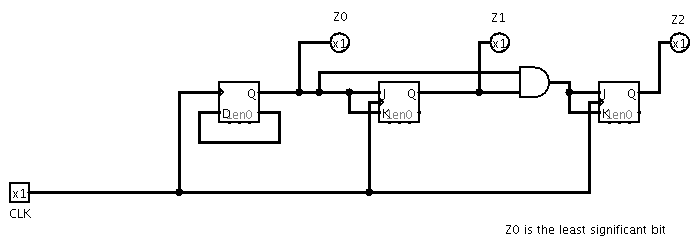
\includegraphics[scale=0.5]{3bit-counter-1D-2JK}
\caption{A 3 bit counter using 1 D flip-flop and 2 JK flip-flops
with bit $Z_0$ as the least significant bit.}\label{fig:circ01}
\end{figure}

To implement this design the circuit diagram should be followed
along with the relevant data sheets for the particular chips.

The following four chips were used during the construction of this lab.

\begin{tabular}{|l|l|}
\hline
74HC74 & dual D flip-flop \\
\hline
74HC109 & dual JK flip-flop \\
\hline
74HC08 & quad 2 input and gates \\
\hline
74HC04 & hex inverting gates \\
\hline
\end{tabular}

Other chips can be substituted but they must all be from the same
family.
CMOS chips cannot be mixed with TTL chips.

On the flip-flops there are additional pins for "reset" and "clear".
These are used to momentarily reset and/or clear the state of the chip.
But in this lab it was not necessary to use them so they were just connected
to hi or low (refer to the data sheet).

The clock inputs to all the chips was the same and was derived from
a switch.
It could also be derived from a function generator.
If a function generator is used the frequency should be reduced
to a value such as 1 hz so that it does not change too fast to be seen.
% }}}

% }}}

% {{{ Observations
\section{Observations}

The 3 bit counter implemented in hardware sequentially counted
from 0 to 7 as expected.
On power up the initial state was not always the same.
This was not a problem in this case since all possibilities were
accounted for but it could be a problem in other situations.
The reset and clear pins could also be used to reset the state
if this was necessary.

% }}}

% {{{ Conclusion
\section{Conclusion}

This lab was a success in designing and implementing a 3-bit binary
counter using D and JK flip-flops.

% }}}

%\renewcommand*{\refname}{\vspace{-8mm}}
%\section{References}
%%%\bibliographystyle{plain}
%%%\bibliographystyle{mslapa}
%\bibliographystyle{ieeetr}
%\bibliography{../references}

\end{document}

% vim:foldmethod=marker
